%!TEX root=paper.tex



  \section{Performance Triangulation With Regression Monitoring}

  Suppose the developer observes a performance degradation of a given API endpoint in the latest version of the system. How do they know whether the degradation is due to the performance of the code, the server load, or the workload mix of the user? 

  \vspace{0.1cm}

  
  One way of triangulating such an observation is by monitoring the evolution of the performance of the endpoints when tested with a constant load across versions. Thus, if the performance decreases in a new version, and the  when an endpoint is tested with a constant load the problem must be the endpoint implementation. 

  \subsection*{Integrating with CI Servers}

  To monitor endpoint performance with a constant load \tool takes advantage of two best practices in software evolution: (1) and API must have unit tests for its endpoints, and (2) these unit tests will be run within a CI server. By tracking the timing of these unit tests one obtains a perspective on endpoint performance evolution with a constant load (as long as the unit tests do not change). 

  \tool can be configured to work together with Continuous Integration (CI) frameworks like Travis\footnote{\url{https://travis-ci.org/}, one of the most popular CI solutions at the moment} that deal with automated integration testing. To do this one needs to simply add one extra line in the script that runs their continuous integration testing. In the case of Travis CI, a developer has to add the following line in `.travis.yml': 


  \begin{lstlisting}[style=custompython]  
# LOC #4: to be added to the .travis.yml file
python -m flask_monitoringdashboard.collect
   --test_folder=./tests_zeeguu_api --times=5 
   --url=https://zeeguu.unibe.ch/api/dashboard

  \end{lstlisting}

  Each time a new build is created through Travis, the \tool automatically detects all available unit tests defined by the application developer (in (-{}-test\_folder)) and iterates through each one of them a number of times (-{}-times) while monitoring the response times for each test. The resulting measurements are uploaded to a specific endpoint that is created by the tool at the API url (-{}-url). The data uploaded to this endpoint is   persisted in a separate part of the tool database so as not to contaminate the ``live'' monitoring data. 

      \begin{figure}[h!]
        \centering
        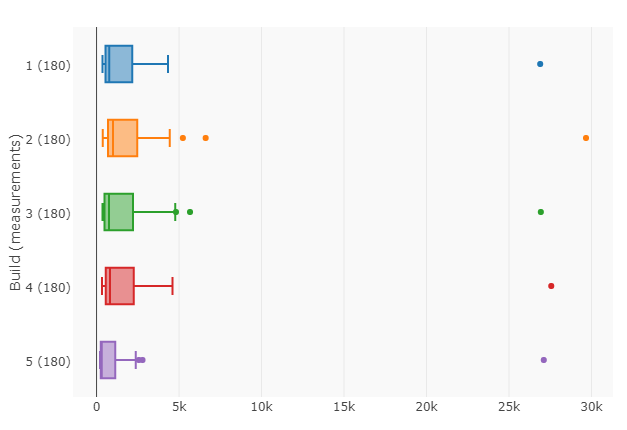
\includegraphics[width=0.45\columnwidth]{travis_builds}
        \caption{Response times in 5 consequent Travis builds}
        \label{fig:builds}
      \end{figure}

  \Fref{fig:builds} is a screenshot from the dashboard showing the measured response times for 5 consequent builds, with 180 iterations of the unit tests executed in total across all endpoints. The outliers on the right of the figure are due to initial requests \ins{which must wait for a boot-up phase of the API}.  
  


  \subsection*{Preemptive Monitoring}
  The concept of {\em preemptive monitoring} of the application performance by means of instrumenting integration unit testing as the synthetic load is similar to the idea of augmenting service monitoring with online testing~\cite{metzger2010proactive}, i.e.~testing service-based applications by using dedicated test input in parallel to its normal use and operation. The difference is that we take advantage of the capability of the CI framework to create an emulated ``live'' environment for integration testing purposes, and use unit testing as the dedicated test input in order to measure performance. 
  
  While this integration testing environment is different from the production one, and the load used is purely synthetic, it can serve as an early performance indicator for the developer.  Figure \ref{fig:response_times_preemptive} shows the actual endpoint response times across five versions of the system (above) and the corresponding testing times for the synthetic load in the same five versions (below). The green line joining the medians hints to a correlation between the two sets of measurements. 

      \begin{figure}[h!]
        \centering
        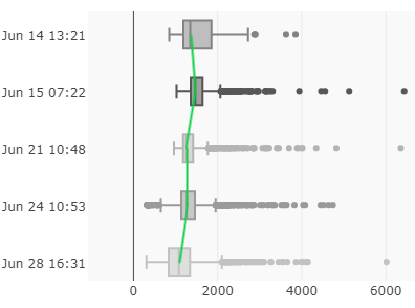
\includegraphics[width=0.75\columnwidth]{response_per_version_trunced_trend}


        \advance\leftskip-0.2cm
        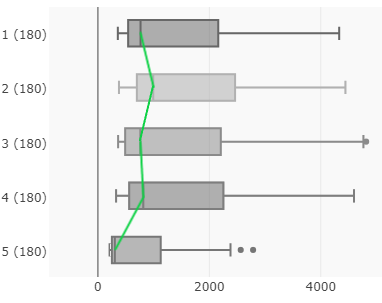
\includegraphics[width=0.5\columnwidth]{travis_builds_no_outliers_trend}
        \caption{The reported response time (in ms) per deployed version in the observation period: 
        in the actual deployment (above) and using integration with Travis (below)}        
        
        \label{fig:response_times_preemptive}
      \end{figure}

  Computing Pearson correlation ($r(3)=.93, p=.02$) between the median values of the two datasets (cf. Table \ref{tab:correlations}) shows that there is a correlation between the two.


    \begin{table}[h]
      
      \centering
      \begin{tabular}{lll}
        \toprule
        Iteration & \bfseries Live (median) & \bfseries Travis (median)\\
        \midrule
        1 & 1349.41 & 764.87\\ 
        2 & 1466.13 & 992.87\\
        3 & 1256.65 & 760.87\\
        4 & 1266.42 & 813.89\\
        5 & 1080.68 & 303.4\\
        \bottomrule
      
      \end{tabular}
      \caption{Median response times in Figure \ref{fig:response_times_preemptive}}
      \label{tab:correlations}
    \end{table}




%   \begin{figure*}[hb!]
%   \centering
%   \subfloat[The reported response time (in ms) per deployed version in the observation period]{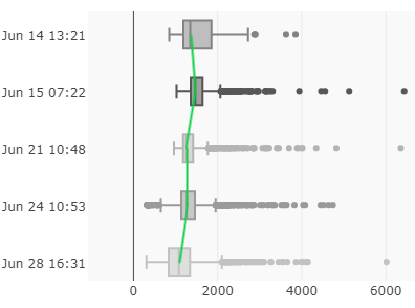
\includegraphics[width=.6\columnwidth]{response_per_version_trunced_trend}}
%   \quad
%   \subfloat[The measured response time (in ms) using integration with Travis]{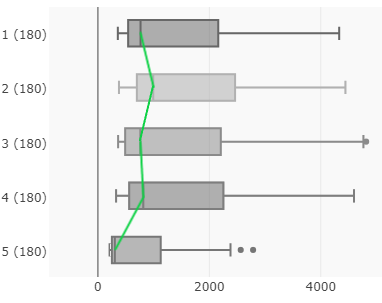
\includegraphics[width=.56\columnwidth]{travis_builds_no_outliers_trend}}
%   \caption{Comparison of the response times per endpoint: actual production system versus preemptive monitoring data}
%   \label{fig:preemptive}
% \end{figure*}

  \ml{This following paragraph is beautifully written, but it's a bit redundant with what it's already said. However maybe after some more refactorings we can put it to use. Worst case, we move it to the conclusion}
  \ins{Besides functioning as an early warning system for performance, tracking the evolving performance of API tests serves a second purpose. To function as an anchor when the developer analyzes performance degradations. For example, when a developer sees that a given endpoint has become less performant after in a newly deployed version, they are able to investigate whether the performance degradation is visible also with the synthetic load. This would correspond to a performance degradation which is due to ``algorithmic performance degradation''. If on the other hand, the performance of the tests does not change between versions, the developer might conclude that the performance degradation could be due to the workload on the machines, or maybe to the workload mix of the users}
  

